\documentclass[12pt,aspectratio=43]{beamer}

%%%%%%%%%%%%%%%%%%%%%%%%%%%%%%%%%%%%%%%%
% Paquetes de configuración basica del %
%               texto                  %
%%%%%%%%%%%%%%%%%%%%%%%%%%%%%%%%%%%%%%%%
\usepackage[spanish,es-nodecimaldot]{babel}
\usepackage[T1]{fontenc}
\usepackage{listings}
\usepackage{hyperref}

%%%%%%%%%%%%%%%%%%%%%%%%%%%%%%%%%%%%%%%%%%%%%
% [listings] Configuración de vizualizacion %
% de código                                 %
%%%%%%%%%%%%%%%%%%%%%%%%%%%%%%%%%%%%%%%%%%%%%
\lstset{
	basicstyle=\ttfamily,
	extendedchars=true,
	showspaces=false,
	showstringspaces=false,
	captionpos=b,
	keywordstyle=\bfseries\color{cyan},
	commentstyle=\color{gray},
	stringstyle=\color{orange},
	escapeinside={!>}{<!} }

%%%%%%%%%%%%%%%%%%%%%%%%%%%%%%%%%%%%%%%%
%  Paquetes de configuración graficos  %
%            del documento             %
%%%%%%%%%%%%%%%%%%%%%%%%%%%%%%%%%%%%%%%%
\usepackage{graphicx}
\usepackage{tikz}
\usetikzlibrary{babel}
\usepackage{xcolor}
\usepackage{pdfpages}

\usepackage{ifxetex}
\ifxetex
	\usepackage[no-math]{fontspec}
	\setmainfont{AncizarSans}[
		Path = ../Fuentes/,
		Extension = .otf,
		BoldFont = *-B,
		ItalicFont = *-I,
		BoldItalicFont = *-BI ]
	\setmonofont{UbuntuMono}[
		Path = ../Fuentes/,
		Extension = .ttf,
		BoldFont = *-B,
		ItalicFont = *-I,
		BoldItalicFont = *-BI ]
	\newcommand{\lmr}{\fontfamily{lmr}\selectfont}
	\newcommand{\lmss}{\fontfamily{lmss}\selectfont}
	\newcommand{\lmtt}{\fontfamily{lmtt}\selectfont}
\fi

%%%%%%%%%%%%%%%%%%%%%%%%%%%%%%%%%%%%%%%%
%      Configuraciones de Beamer       %
%%%%%%%%%%%%%%%%%%%%%%%%%%%%%%%%%%%%%%%%
\definecolor{Igreen}{RGB}{148,180,59}
\definecolor{Ired}{RGB}{166,24,49}
\setbeamertemplate{navigation symbols}{}

\usefonttheme{professionalfonts}
\usefonttheme{serif}
\setbeamercolor{frametitle}{fg=Ired,bg=Igreen!50}

%%%%%%%%%%%%%%%%%%%%%%%%%%%%%%%%%%%%%%%%
%    Información de la presentación    %
%%%%%%%%%%%%%%%%%%%%%%%%%%%%%%%%%%%%%%%%
\title{Introducción a {\lmr\LaTeX}}
\author{Joar Esteban Buitrago Carrillo}
\institute{Universidad Nacional de Colombia}
\date{}

\defbeamertemplate*{title page}{customized}[1][]
{
	\vfill
	\begin{center}
		{\Huge\inserttitle}\\
		\bigskip
		{\Large Curso Libre de {\lmr\LaTeX}}\\
		\bigskip
		\insertauthor\\[10pt]
	\end{center}
	\vfill
	
\includegraphics[height=1cm]{../Escudo_UN}\hspace{0.25cm}
}

\begin{document}
\maketitle

{
	\setbeamercolor{background canvas}{bg=}
	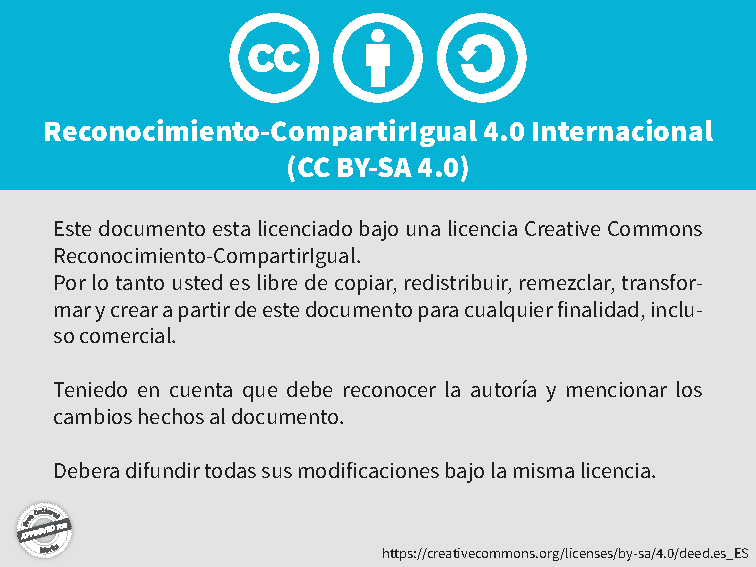
\includepdf{../Licencia_Diapositiva.pdf}
}

\begin{frame}{¿Que es {\lmr\LaTeX}?}{}
{\lmr\LaTeX} es un sistema de composición de textos de calidad artística y tipográfica. Es usado muy habitualmente en el mundo científico debido a todas sus características y facilidad de trabajo.\pause\\[2em]
	
{\lmr\LaTeX} es un conjunto de macros de {\lmr\TeX}, licenciado bajo la licencia {\it{\lmr L}PPL}, {\it{\lmr\LaTeX} Project Public License}. Por lo cual es {\em Software Libre} y gratuito.
\end{frame}

\section{Clases}

\section{Estructura del código}

\section{Títulos}

\section{Capitulos-Partes, Secciones, etc.}

\section{El resumen}

\section{Estilos, Familias y Formas}

\section{Tamaño de fuente}

\section{Paquetes \lstinline[language=[LaTeX]TeX]|fontenc| e \lstinline[language=[LaTeX]TeX]|inputenc|}

\section {{\lmr\LaTeX} en español}

\section{Separación del texto}

\section{Opciones del Documento}
\end{document}
